\documentclass[a4paper,12pt]{article}

\usepackage{estilos}

\pagestyle{empty}

\begin{document}
\begin{center}%
\begin{figure}[H]%
\hspace*{-.2in}{\begin{minipage}[H]{.5\columnwidth}%
\centering%
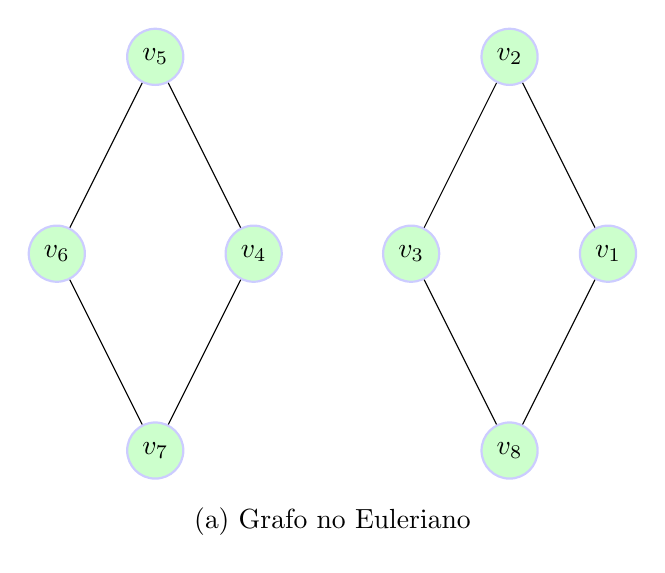
\begin{tikzpicture}{node distance=1.3cm,>=stealth',bend angle=45, auto}
  \tikzstyle{place}=[circle,thick,draw=blue!20,fill=green!20,minimum size=6mm]
  \tikzstyle{texto}=[]

  \begin{scope}

    \node [place] (c1) [xshift=-20cm]{$v_6$};

    \node [place] (c2) [right of=c1,xshift=.25cm,yshift=2.5cm] {$v_5$}
    edge [] (c1);

    \node [place] (c3) [right of=c1,xshift=.25cm,yshift=-2.5cm] {$v_7$}
    edge [] (c1);

    \node [place] (c4) [right of=c1,xshift=1.5cm] {$v_4$}
    edge [] (c2)
    edge [] (c3);

    \node [place] (c5) [right of=c4,xshift=1cm] {$v_3$};

    \node [place] (c6) [right of=c5,xshift=.25cm,yshift=2.5cm] {$v_2$}
    edge [] (c5);

    \node [place] (c7) [right of=c5,xshift=.25cm,yshift=-2.5cm] {$v_8$}
    edge [] (c5);

    \node [place] (c8) [right of=c5,xshift=1.5cm] {$v_1$}
    edge [] (c6)
    edge [] (c7);

    \node [texto] (p1) [below of=c7,yshift=.1cm,xshift=-2.25cm] {(a) Grafo no Euleriano};
  \end{scope}
\end{tikzpicture}
\end{minipage}}
\hspace*{.2in}{ \begin{minipage}{3cm}
\begin{center}
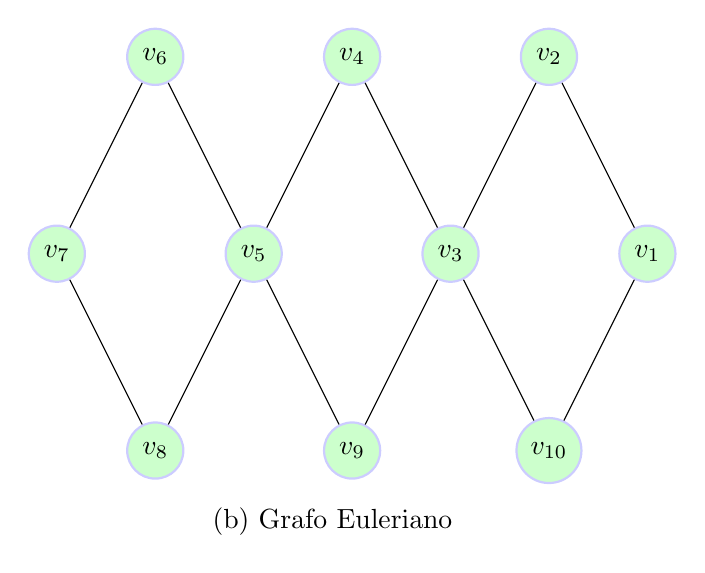
\begin{tikzpicture}{node distance=1.3cm,>=stealth',bend angle=45,auto}

  \tikzstyle{place}=[circle,thick,draw=blue!20,fill=green!20,minimum size=6mm]
  \tikzstyle{texto}=[]

  \begin{scope}


    \node [place] (t1) {$v_7$};

    \node [place] (t2) [right of=t1,xshift=.25cm,yshift=2.5cm] {$v_6$}
    edge [] (t1);

    \node [place] (t3) [right of=t1,xshift=.25cm,yshift=-2.5cm] {$v_8$}
    edge [] (t1);

    \node [place] (t4) [right of=t1,xshift=1.5cm] {$v_5$}
    edge [] (t2)
    edge [] (t3);

    \node [place] (t5) [right of=t4,xshift=1.5cm] {$v_3$};

    \node [place] (t6) [right of=t5,xshift=.25cm,yshift=2.5cm] {$v_2$}
    edge [] (t5);

    \node [place] (t7) [right of=t5,xshift=.25cm,yshift=-2.5cm] {$v_{10}$}
    edge [] (t5);

    \node [place] (t8) [right of=t5,xshift=1.5cm] {$v_1$}
    edge [] (t6)
    edge [] (t7);

    \node [place] (t9) [right of=t4,xshift=.25cm,yshift=2.5cm] {$v_4$}
    edge [] (t4)
    edge [] (t5);

    \node [place] (t10) [right of=t4,xshift=.25cm,yshift=-2.5cm] {$v_9$}
    edge [] (t4)
    edge [] (t5);

    \node [texto] (p1) [below of=t7,yshift=.1cm,xshift=-2.75cm] {(b) Grafo Euleriano};


\end{scope}

\end{tikzpicture}

\end{center}
\end{minipage}}
\end{figure}
\end{center}
\end{document}
